\chapter{Language for Run-time State Migration}
\label{ch:language}
As stated by \textbf{R2 Platform-independent State Specification}, need a platform-independent representation of run-time state. For this, we develop a language to describe run-time states. The requirements for this language are on the requirements D1 to D3 (Chapter \ref{ch:requirements}).
In this chapter, the DSL definition and interpretation, specification of run-time state, and terminology used are described.
% This includes the interpretation which defines the semantics, meta-model description which describe the abstract syntax, run-time state specification which is the definition of the concrete syntax, and some run-time state specification examples.
The definition of the language occurs on different layers (Figure \ref{fig:asml}). On the top layer, we define a language for specify a type of state an application. Such a specification of a specific type of state resides on the middle layer. Concrete instances of this type, a specific run-time state of an application, is located on the bottom layer. All three layers are explained subsequently.

\FloatBarrier
\begin{figure}[H]
    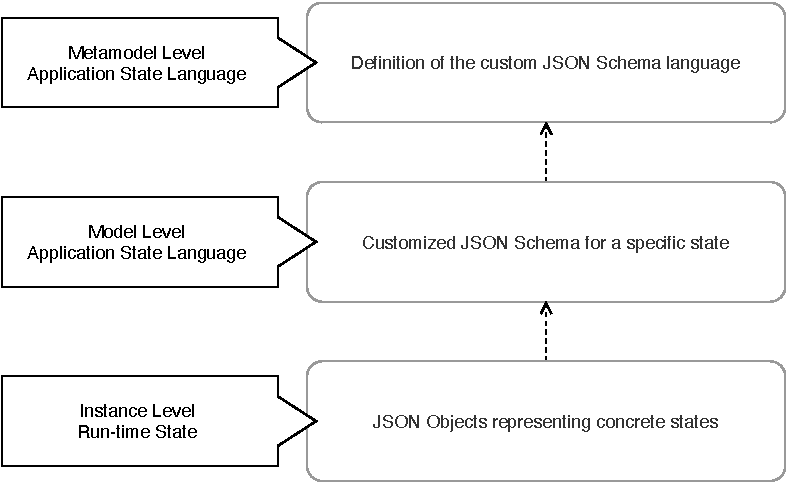
\includegraphics[scale=0.8]{../figures/asml.pdf}
    \centering
    \caption{The definition of the language on different layers.}
    \label{fig:asml}
\end{figure}
\FloatBarrier


\section{Application State Modeling Language}
After research and looking for suitable existing state modeling languages, it has been decided to create a new DSL based on run-time state migration requirements. A Domain-specific language (DSL) can be developed from scratch, or it can be a modification or a restricted form of an existing modeling language.

The Application State Modeling Language (ASML) is a DSL that defines each state of any software application. The focus of this language is on modeling states of the run-time.

An application can have multiple states. This language allows developers to write a custom model. Each model covers an individual state. 

As mentioned in requirements (Chapter \ref{ch:requirements}), this language supports states that are migratable. It is not supporting the transition between states as we assume we know in which state application is.

The advantage of having an individual model for each state is improving interoperability, allowing different domain applications to share a specific part of them. For example, an email domain application has a calendar that can migrate data with a phone calendar application.


\subsection{Language Stack}
There are so many ways to define a DSL; it can be made from scratch (e.g., developing a language base on Xtext framework) or extended or restricted versions of other languages. The ASML is introduce a syntax based of JSON and is a restricted version of JSON Schema.

\subsubsection{JSON}
JSON (JavaScript Object Notation) is a file format. It is lightweight and human-readable text to store and transmit data based on the data types of the JavaScript programming language. In the last few years, many programming languages are supporting JSON, which gained popularity among developers, and has become the primary data format for exchanging information \cite{json-schema}. JSON documents consist of attribute-value pairs, which the value can be again a JSON document and there is not limit of the nesting level. A simple JSON documents is shown in Listing \ref{lis:json}.

\lstset{
  label=lis:json, caption=A simple JSON document., 
  basicstyle=\ttfamily\footnotesize, frame=single, captionpos=b,
  xleftmargin=.15\textwidth, xrightmargin=.15\textwidth
}
\begin{lstlisting}
{
    "fullname": "John Doe",
    "email": "john@mail.upb.de"
}
\end{lstlisting}

\subsubsection{JSON Schema}
After the tremendous popularity of JSON, some scenarios could benefit from a declarative way of defining a schema for JSON documents. A declarative schema specification would give programming languages and also developers a standardized language to specify what types of JSON documents are valid as inputs and outputs \cite{json-schema}.

The schema can be another JSON document which defines acceptable attribute-value pairs. For instance, the simple JSON document in Listing \ref{lis:json}, can be declare in JSON schema document in Listing \ref{lis:json-schema}

\lstset{
  label=lis:json-schema, caption=A simple JSON schema document., 
  basicstyle=\ttfamily\footnotesize, frame=single, captionpos=b,
  xleftmargin=.15\textwidth, xrightmargin=.15\textwidth
}
\begin{lstlisting}
{
    "properties": {
        "fullname": {
            "type": "string"
        },
        "email": {
            "type": "string",
            "format": "email"
        }
    }
}
\end{lstlisting}


\subsection{Language Schema}
description of the schema of the ASML.

\begin{itemize}
\item title
\item description
\item version
\item properties
\item required
\item additionalProperties
\item definitions
\end{itemize}

\subsection{Data Types}
here are data type of the ASML.


\begin{itemize}
\item array
\item boolean
\item integer
\item number
\item object
\item string
\item null
\end{itemize}


\section{Application State Model}

The Application State Model is a JSON Schema document that defines what a state must contain at run-time and is validated against Application State Modeling Language. To enable run-time state migration, developers should write a custom Application State Model (or use an existing one) for a run-time state in a JSON Schema document.

Any application has different states; Each state should have its own model, which is a JSON Schema document. At the time of integration, Application State Models must be coupled with the source and target applications to determine which states are available for migration.

For migration to happen, source and target applications must have a common Application State Model. As each state is modeled individually, different domain application with the same-purpose part can migrate their states. For example, an e-mail client has a to-do list feature which can be a standard characteristic for a task management application. So, they have some common states like writing a task and searching.

Developers can write their own Application State Model or using the existing ones. Variables of a run-time state that need to be migrated shall be identified and associated to keywords. As stated in requirement \textbf{R3 Model Repository}, we made a repository manager call "model-repository" located on GitHub \footnote{\href{https://github.com/asml-lang/model-repository}{https://github.com/asml-lang/model-repository}}. Some models are available on this repository. Developers can look into the repository and search for these keywords to find a suitable model for their application. They may use an existing one or even extending it by making a new model. To write a new model, variables of a run-time state which they are associated to some keywords should be specified by their name, type or their format. For example, when a search state needs to be migrated, we need to migrate a text and maybe the submission status. These variables can be associate with some keywords like "query" as a string and "submit" as a boolean. These associated keywords and their type must be specified in \lstinline[basicstyle=\ttfamily]{properties} section of Application State Model which is described in next section. 

After making a new model, developers can add it the repository manager by making a pull request. So, other developers may use it for their applications.

\subsection{Top-level Fields}
There are some fields that they need to be in an Application State Model to define a state’s specification.

\subsubsection{asml}
As stated in requirement\textbf{D3 Validating}, a model must have an object field named “asml” whose string value represents the version of ASML. This version follows SemVer pattern \footnote{\href{https://semver.org/}{https://semver.org/
}} and helps to validate the model against the correct version of our DSL. Listing \ref{lis:asm-asml} shows how the “asml” field has to be defined. The version of ASML in this Application State Model is “1.0.0”.

\lstset{
  label=lis:asm-asml, caption=Application State Model “asml” field example., 
}
\begin{lstlisting}[language=yaml]
asml: 1.0.0
\end{lstlisting}
\subsubsection{info}
As stated in requirement \textbf{D2 Finding Same Model}, a model must have an object field named “info” whose object value represents the basic model’s information. This object must have two string values “title” and “version”. Also, “keywords” is an array of string which should contains some keywords that other developers can find this model in Model Repository. Common models can be fined and distinguished by values of “title”, “version” and  “keywords”. Other fields are “description” and “contact”, which are optional. The “description” is a string value that represents the descriptive text about the purpose of the model, and “contact” is the author’s information in case of further contacts. Listing \ref{lis:asm-info} shows an example of how the “info” field has to be defined.

\lstset{
  label=lis:asm-info, caption=Application State Model “info” field example. 
}
\begin{lstlisting}[language=yaml]
title: sending-email
description: A schema model for sending an email
version: 1.0.0
keywords:
- email
- e-mail
- compose
contact:
  name: Saman Soltani
  email: saman@mail.upb.de
  url: samansoltani.com

\end{lstlisting}

\subsubsection{properties}
A model must have an object field named “properties” whose object value represents a state’s specification. Based on ASML, any element of the “properties” object is considered a variable that can be migrated.
Listing \ref{lis:asm-properties} shows an example that has four fields with different types such as from, to, subject and body. These fields should be in the state.

\lstset{
  label=lis:asm-properties, caption=Application State Model “properties” field example.
}
\begin{lstlisting}[language=yaml]
properties:
  from:
    type: string
    format: email
  to:
    type: array
    items:
      type: string
      format: email
  subject:
    type: string
  body:
    type: string

\end{lstlisting}
\subsubsection{required}
As stated in requirement \textbf{D1 State Specification}, a model can have an object field named “required” which its array of strings value represents compulsory variables in the state.
Listing \ref{lis:asm-required} shows an example which has three string value in an array. These fields must exist in the state as they are specified in “required” field.

\lstset{
  label=lis:asm-required, caption=Application State Model “required” field example.
}
\begin{lstlisting}[language=yaml]
required:
- from
- to
- body

\end{lstlisting}

\subsection{Example Models}
\subsubsection{Composing New E-mail}
Considering an e-mail client application in which the user can write an e-mail. The state of composing a new e-mail can have a minimum of four fields which are “from”, “to”, “subject” and “body”. A combination of Listings \ref{lis:asm-asml},  \ref{lis:asm-info},  \ref{lis:asm-properties} and  \ref{lis:asm-required} shows an example of this model.
The complete version of the Application State Model of composing a new e-mail is shown in Listing \ref{lis:sending-email-schema}.
\subsubsection{Writing Note}
Considering a note-taking application that has only one state for migration which is writing a note. It can be modeled with a compulsory “text” string field as in Listing \ref{lis:note-schema}.

\lstset{
  label=lis:note-schema, caption=Note Writing example Application State Model as JSON Schema in YAML.
}
\begin{lstlisting}[language=yaml]
asml: 1.0.0
info:
  title: writing-note
  version: 1.0.0
properties:
  text:
    description: content of the note
    type: string
required:
- text

\end{lstlisting}
\subsubsection{Search}
Searching between data is very common between applications. If there would a search feature; Also, there is a search result. The search state can be modeled so that the application knows if the search has been submitted by the user or not; it can adjust itself base on a received state. The search model can have a compulsory “query” string field, which defines the text that the user is looking for, and a “submit” boolean field shows if the search has been submitted.

This Application State Model can be used in different purpose applications which they have the search feature. Listing \ref{lis:search-schema} shows a search state modeled defined as Application State Model in a JSON Schema document.

\lstset{
  label=lis:search-schema, caption=Search example Application State Model as JSON Schema in YAML.
}
\begin{lstlisting}[language=yaml]
asml: 1.0.0
info:
  title: search
  version: 1.0.0
properties:
  query:
    description: the query of search
    type: string
  submit:
    description: shows if the query is already has been submitted
    type: boolean
required:
- query
\end{lstlisting}

\section{Run-time State}
The Run-time State is a JSON document which contains the actual attribute/values of a state. Run-time State is validated against Application State Model, if the state is valid, it can be migrated from source to target application.
Target application should adjust itself with new state.

\subsection{Example Run-time States}

\subsubsection{Composing New E-mail}
Based on composing new e-mail Application State Model (Listing \ref{lis:sending-email-schema}) valid example values for sending e-mail state is shown in Listing \ref{lis:sending-email-state}.

\lstset{
  label=lis:sending-email-state, caption=A Run-time State for sending e-mail as JSON document., 
  basicstyle=\ttfamily\footnotesize, frame=single, captionpos=b,
  xleftmargin=.15\textwidth, xrightmargin=.15\textwidth
}
\begin{lstlisting}
{
  "from": "engels@uni-paderborn.de",
  "to": [
    "saman@mail.upb.de",
    "dennis.wolters@upb.de"
  ],
  "subject": "Master Thesis Grade",
  "body": "Dear Saman\n, Your master thesis grade is 1.0."
}
\end{lstlisting}


\subsubsection{Writing Note}
Based on writing note Application State Model (Listing \ref{lis:note-schema}) valid example values for writing note state is shown in Listing \ref{lis:writing-note-state}.
 
\lstset{
  label=lis:writing-note-state, caption=A Run-time State for writing note as JSON document., 
  basicstyle=\ttfamily\footnotesize, frame=single, captionpos=b,
  xleftmargin=.15\textwidth, xrightmargin=.15\textwidth
}
\begin{lstlisting}
{
    "text": "example text"
}
\end{lstlisting}

\subsubsection{Search}
Based on search Application State Model (Listing \ref{lis:search-schema}) valid example values for search state is shown in Listing \ref{lis:search-state}.
\lstset{
  label=lis:search-state, caption=A Run-time State for search as JSON document., 
  basicstyle=\ttfamily\footnotesize, frame=single, captionpos=b,
  xleftmargin=.15\textwidth, xrightmargin=.15\textwidth
}
\begin{lstlisting}
{
    "query": "example text",
    "submit": true
}
\end{lstlisting}